\documentclass[12pt, a4paper]{ctexart}

% -----------------------------------------------------------
% 宏包引入
% -----------------------------------------------------------
\usepackage{geometry}       % 页面布局
\usepackage{fancyhdr}       % 页眉页脚
\usepackage{setspace}       % 行间距
\usepackage{xcolor}         % 颜色支持
\usepackage{graphicx}       % 图片支持
\usepackage{caption}        % 标题样式
\usepackage{wrapfig}        % 【核心】实现图文绕排
\usepackage{calc}           % 计算宽度

% -----------------------------------------------------------
% 页面设置
% -----------------------------------------------------------
% 左右边距稍微调窄一点，给“左文右图”留出足够空间
\geometry{
    top=3.0cm,
    bottom=3.0cm,
    left=2.5cm,
    right=2.5cm
}

% 定义颜色
\definecolor{DeepBlue}{RGB}{25, 25, 112} % 深午夜蓝
\definecolor{GrayText}{RGB}{80, 80, 80}  % 灰色辅助文字
\definecolor{AccentRed}{RGB}{160, 50, 50} % 强调色

% 图片路径 (根据您之前的要求设置)
\graphicspath{{../../images/sw/rssh/}}

% 行间距
\linespread{1.5}

% -----------------------------------------------------------
% 页眉页脚
% -----------------------------------------------------------
\pagestyle{fancy}
\fancyhf{} 
\fancyhead[L]{\kaishu \small \textcolor{GrayText}{且去温习那场暴雨}} 
\fancyhead[R]{\kaishu \small \textcolor{GrayText}{生命感悟}} 
\fancyfoot[C]{\thepage} 
\renewcommand{\headrulewidth}{0.4pt} 

% -----------------------------------------------------------
% 自定义命令
% -----------------------------------------------------------
% 思想强调样式
\newcommand{\thought}[1]{{\kaishu \color{DeepBlue} #1}}

% 图片标题样式：右对齐，灰色，小字
\captionsetup{labelformat=empty, justification=raggedleft, font={small, color=GrayText}, singlelinecheck=false}

\begin{document}

% -----------------------------------------------------------
% 标题部分
% -----------------------------------------------------------
\begin{center}
    \vspace*{0.5cm}
    {\Huge \bfseries \textcolor{DeepBlue}{随笔：且去温习那场暴雨}}
    \vspace{0.5cm}
    \noindent\makebox[\linewidth]{\rule{10cm}{0.4pt}} 
    \vspace{1.0cm}
\end{center}

% -----------------------------------------------------------
% 正文与图片开始
% -----------------------------------------------------------

% 【第一张图】放在右侧，图文绕排
\begin{wrapfigure}{r}{0.45\textwidth}
    \vspace{-20pt} % 向上微调，对齐首行
    \centering
    % 使用您文件夹中的图片
    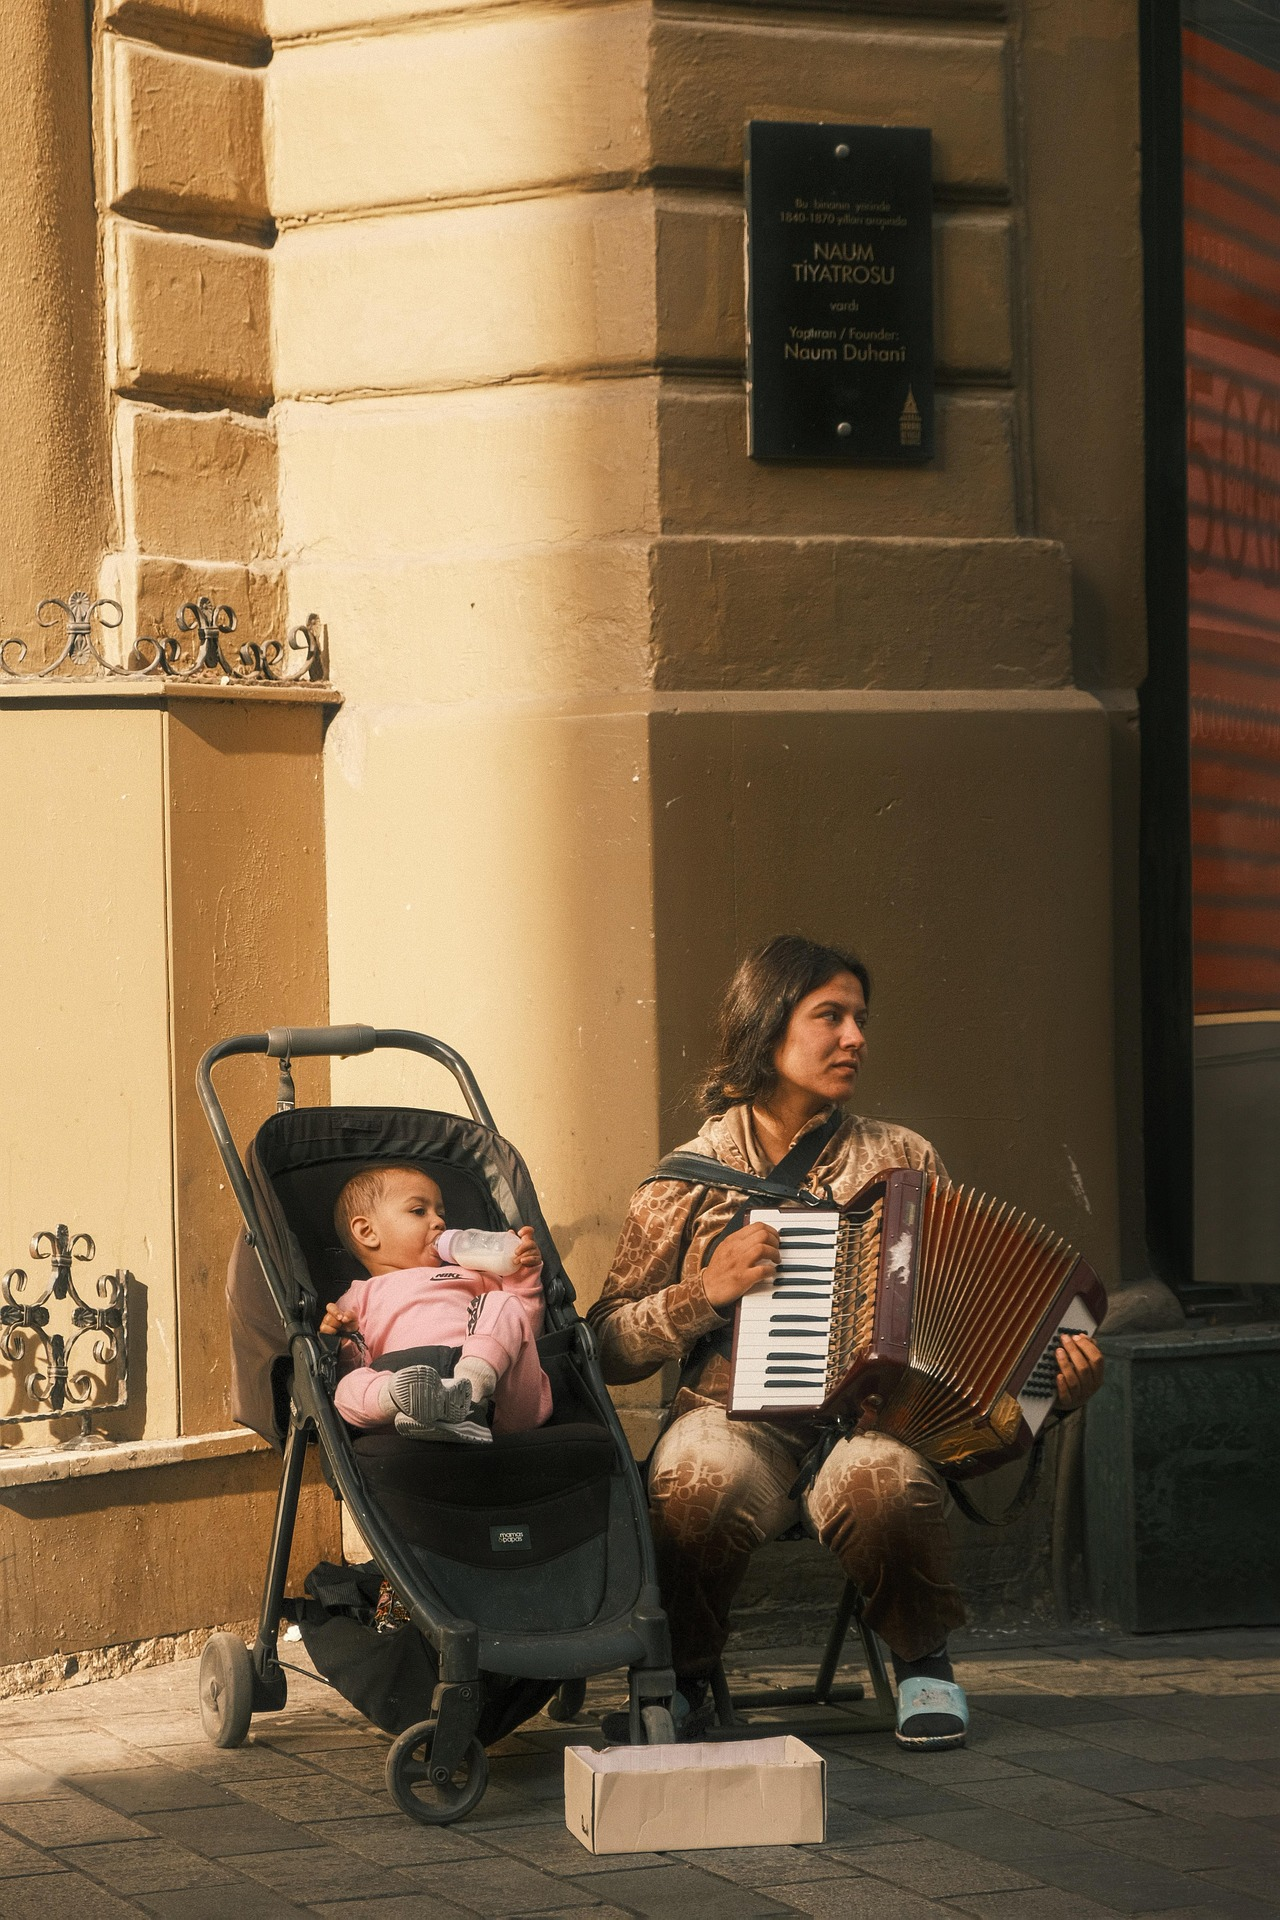
\includegraphics[width=\linewidth]{people-7707981_1920.jpg}
    \caption{生命螺旋，周而复始}
    \vspace{-10pt} % 减少下方空白
\end{wrapfigure}

今天在赶了几篇课设论文时候，我脑子里对于一个一直指导我人生的思想逐渐明朗，在这一下，想要分享给大家的这个欲望一下子涨起来了。首先我给今天我要分享的观点命名一下，我把它命名为：\textbf{\textcolor{DeepBlue}{“周期性课题守恒律”}}。这是我在接触斯多葛学派的坚忍、阿德勒心理学的勇气，以及马克思辩证唯物主义的发展观之后，基于我自己的一些日常事宜以及经历的感受，把他们融合在一起的一个概念。

首先，我眼中的人生——也就是我们每个人这几十年的所见、所闻、所感，它绝不是一段无序的随机漫步，而是一个\textbf{分阶段、有规律、螺旋式上升}的动态过程。在这里呢，我要特别澄清一点：我并非在鼓吹宿命论，也不是说所有人都要活成同一个模子或者是说大家都会是同种感悟。每个人的人生剧本都是独一无二的，那些自己经历的悲欢离合、那些每一次让你大哭或者大笑的瞬间，这都属于你自己，这也一定是不可复制至其他人的。

但我真正想要表达的是：\thought{“虽然我们的‘体验形式’以及‘过程’千差万别，但在生命的螺旋进程里，那些必须面对的‘课题’却是不可逾越的，必然是守恒的。”}

人这一辈子，是分周期的。在特定的年龄段，或者说在那个特定的螺旋层级上，命运一定会给你派发特定的考卷。无论你是谁，关于自我接纳、关于亲密关系、关于责任承担、关于生老病死，这些课题都会准时的在你的人生周期降临。这便是我所说的关于人生的“\textbf{必然体验}”。

面对这些必然降临的挑战，人们大多数都会试图逃避，这与我们几万年的进化中“省力”是对应一致的。可是我们大家都知道的事，一些你不愿意直接面对的事情，譬如“工作受阻”、“家庭关系不和睦”、“学业不顺利”等等，这些你没有在当下阶段解决的课题，那它一定会重新出现在你后续的其他阶段，这是无法逃避的。

\begin{wrapfigure}{l}{0.4\textwidth} % 这里换到左侧绕排，增加版面变化
    \vspace{-10pt} 
    \centering
    % 如果没有第二张图，可以重复使用一张，或者去掉 wrapfigure
    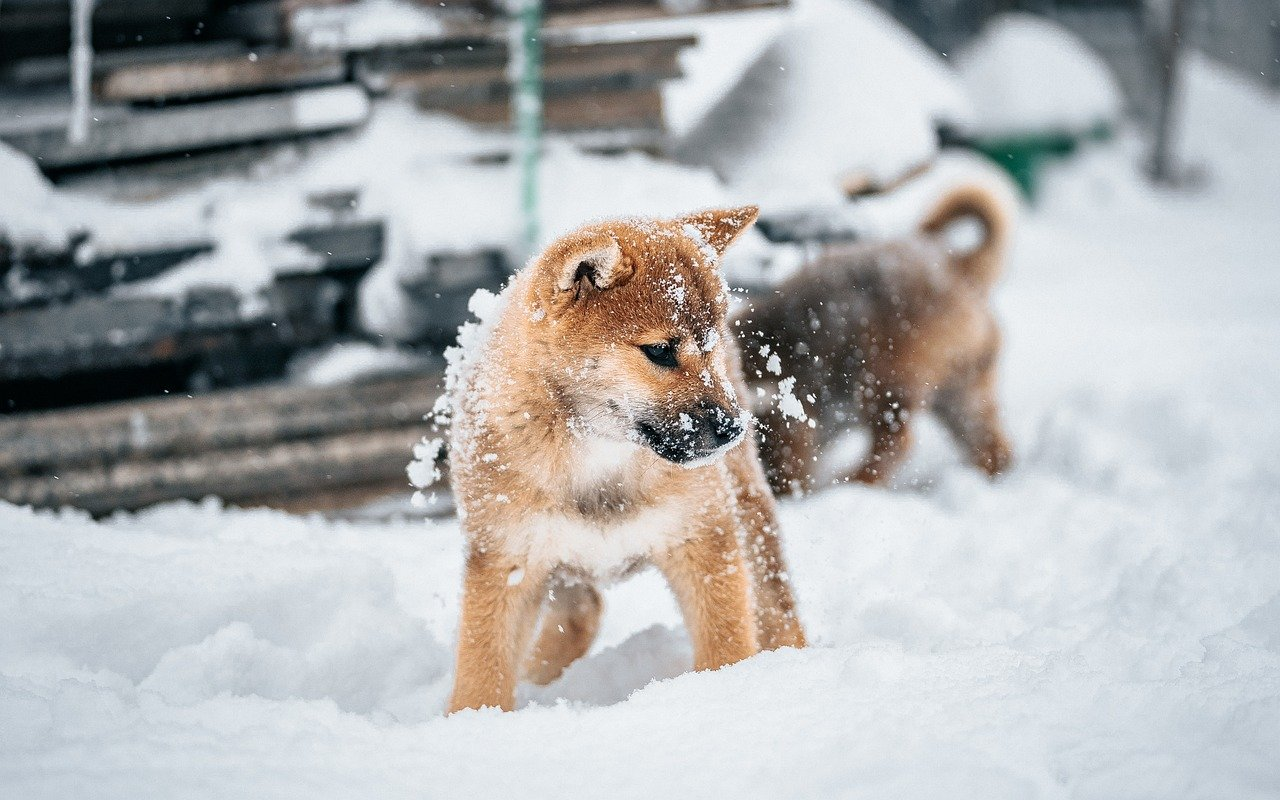
\includegraphics[width=\linewidth]{dog-9830833_1280.jpg} 
    \caption{}
    \vspace{-10pt} 
\end{wrapfigure}

人生中必须经历的体验总是守恒的。那些你此刻因为恐惧而试图绕过的课题、那些你想要逃避的责任，它们并不会凭空消失，也不会被岁月冲淡。它们只是暂时让你觉得安好，但其实这个就像高息借贷，这些“体验债务”会一直积压在你人生的账户里，并且在后续让你付出更高的代价。

也就是说：如果你现在不全身心、勇敢地去经历它、去克服它、去感受那份痛苦或磨砺，那么在未来的某一个人生周期，这些未完成的课题终将以更猛烈的程度复现。

二十岁逃避的磨练，三十岁会变成危机；三十岁逃避的责任，四十岁会变成崩塌。

所以，这就是我在本文中想要对自己，也对所有人分享的话：\thought{“面对人生那些必然的课题，请全身心地去‘体验’吧。既然不可逾越，那就正面硬刚；既然守恒存在，那就当下结清。”}

唯有彻底地面对、经历它，我们才能真正翻过这一页，去迎接生命螺旋中的下一次上升。

\vspace{2cm}
\begin{center}
    \textit{\textcolor{GrayText}{—— end ——}}
\end{center}

\end{document}
